\documentclass[conference]{IEEEtran}
\IEEEoverridecommandlockouts
% The preceding line is only needed to identify funding in the first footnote.
% If that is unneeded, please comment it out.
% ICCIT 2026 submission draft (based on the IEEE conference template,
% template version as of 6/27/2024).
% Offline Bangla Disaster-Response Question Answering with Compact
% Open-Source LLMs: a CPU-Only Accuracy-Safety-Efficiency Evaluation

\usepackage{cite}
\usepackage{amsmath,amssymb,amsfonts}
\usepackage{algorithmic}
\usepackage{graphicx}
\usepackage{textcomp}
\usepackage{tikz}
\usetikzlibrary{arrows.meta,positioning,shapes.geometric,fit}
\usepackage{xcolor}
\usepackage{booktabs}
\usepackage{array}
\usepackage{url}
\usepackage{multirow}
\graphicspath{{figures/}}
\urlstyle{same}
\def\BibTeX{{\rm B\kern-.05em{\sc i\kern-.025em b}\kern-.08em
    T\kern-.1667em\lower.7ex\hbox{E}\kern-.125emX}}

\begin{document}

\title{Offline Bangla Disaster-Response Question Answering with Compact Open-Source LLMs:\\ A CPU-Only Evaluation of Accuracy, Safety, and Efficiency Trade-offs}
\maketitle

\begin{abstract}
Disaster-response question answering (QA) in low-resource languages such as Bangla is often required where connectivity is unreliable, so only small, offline, open-weight models can run on local hardware. We benchmark six compact models under 4B parameters (four instruct, two Bangla base) on a new 634-item Bangla disaster-answer QA set spanning 24 categories, plus a 64-item adversarial answerability probe, all served offline on a consumer CPU (8 GB RAM). Accuracy uses a multilingual cross-encoder at a deliberately strict threshold ($t=0$), calibrated against 2{,}058 human correctness labels and cross-validated against chance (0\%) and verbatim-gold (100\%) anchors. We find that no compact offline model is currently trustworthy for autonomous deployment: the best
CE accuracy is only 25.7\% (Qwen3-4B-Instruct; 24.8\% on a hazard-balanced subset), and on unanswerable or
false-premise items 62.5--93.8\% of answers were confident over-answers rather than safe refusals, with the two Bangla base models worst on safety despite mid-pack accuracy. Accuracy and safety largely track model family and instruction tuning rather than
size, while efficiency spans $0.8$--$62.2$ s per answer and 917--3{,}572 MB peak RAM. We release the
dataset, adversarial set, and scoring pipeline as a reproducibility base.
\end{abstract}

\begin{IEEEkeywords}
Bangla NLP, disaster response, large language models, offline inference, safety evaluation
\end{IEEEkeywords}

\section{Introduction}
Bangladesh is one of the most disaster-prone countries in the world: annual floods and cyclones
displace tens of
millions of people and routinely sever both the power grid and cellular connectivity in the affected
regions. In these hours an affected family's most urgent questions are concrete and locally
specific, and the channels best equipped to answer them (remote APIs, web search, official
helplines) collapse first, leaving only a low-end laptop or Android phone, intermittent power, and
no route to a server. Any system that answers disaster questions in this setting must therefore be
\emph{accurate} when a verified answer exists, \emph{safe}---willing to decline---when none does,
and \emph{cheap enough} to run on that hardware without a network.

Compact open-weight large language models (LLMs) that run entirely on a single offline device are an obvious
candidate, and the past two years have produced a steady stream of sub-4B checkpoints, from Bangla-specialised
bases such as TituLLMs~\cite{titullm} to general-purpose instruction releases such as the
Qwen3 and Gemma3 checkpoints evaluated here. Whether
any is \emph{good enough} for unattended deployment is not settled by the multilingual leaderboards
that dominate
public evaluation. Three properties are needed simultaneously---accuracy on answerable questions,
safety on unanswerable or misleading ones, and low latency and memory on CPU-only hardware---and
each is exactly what mainstream evaluation omits: general benchmarks are English-centric and
quiz-like, published latency figures assume GPU acceleration and conflate cold start with
steady-state decoding, and accuracy is rarely paired with an answerability axis---so a model can top
a leaderboard while inventing a first-aid instruction.

Existing Bangla NLP resources stop at classification, span extraction, or instruction-following QA, and
disaster-response NLP is confined to social-media triage~\cite{disastermultimodal}. The gap is not a
missing model but a missing \emph{protocol}: without a hazard-domain benchmark, a human-calibrated
scoring rule, and an explicit answerability axis, the offline-deployment question cannot be
answered, because any single-axis score can be maximised by a model that is dangerous to use. The
question we ask is
therefore empirical: \emph{can a sub-4B open-weight model, served with neither cloud access nor a GPU, be both
accurate and safe enough to support offline disaster-response QA in Bangla, and what does it cost in
latency and
memory?}

We answer it with a controlled, fully offline evaluation: a curated benchmark with per-item safety
labels plus an adversarial answerability probe, a strict human-calibrated cross-encoder scoring
threshold, hand labels for every adversarial output, and six compact open-weight models evaluated
end-to-end on an 8~GB CPU-only laptop (Figure~\ref{fig:flow}). Accuracy, safety, and
efficiency are measured on the same items in the same run, so the three axes can be traded off
rather than reported in isolation. This paper contributes three things.

\begin{enumerate}
\item \textbf{A human-curated Bangla disaster-response QA benchmark with an explicit safety and answerability
axis.} We release 634 Bangla question--answer pairs spanning 24 hazard and response categories
(flood, cyclone,
lightning, heat wave, drinking-water safety, first aid, livestock), distilled from 154 facts taken from 116
official or institutional sources such as the Bangladesh Meteorological Department, the Directorate General of
Health Services, and the Fire Service. Every item carries a \emph{low}/\emph{medium}/\emph{high} safety label
marking how dangerous a wrong answer would be, while macro and hazard-group-balanced views stop the
deliberately flood-heavy distribution from dictating the conclusions. Alongside it we release a
64-item \emph{adversarial answerability probe} of four trap types---unanswerable specifics, false
premises, out-of-scope requests, unknowable predictions---for which the only correct behaviour is to
refuse or correct the premise. To our knowledge this is the first generative, human-verified QA
resource for Bangla disaster guidance.

\item \textbf{A strict, human-calibrated accuracy and safety protocol that makes the numbers auditable.} We
define a model answer to be \emph{correct} when a multilingual cross-encoder relevance score exceeds a fixed
threshold $t=0$, and we justify rather than tune it: 2{,}058 human correctness labels show that tuning $t$ on the
labelled rows is invalid, a wrong-gold (chance) condition passes 0 of 400 pairs, and verbatim gold passes 634 of
634, so $t{=}0$ is a conservative lower bound whose conservatism is itself measured (59.2--71.7\% agreement with
human verdicts). On the safety side a Bangla refusal/over-answer lexicon gives an automatic first pass, but
because lexicons are imperfect \emph{every} adversarial output (6 models $\times$ 64 items $=384$) is hand-labelled,
with an independent re-label of a stratified 32-row sample (84.4\% agreement, Cohen's $\kappa=0.774$). We also
introduce \emph{over-answering}---confident fabrication where declining was correct---as a measurable failure mode.

\item \textbf{A three-axis efficiency--accuracy--safety evaluation of six compact models on CPU-only hardware,
plus a deployment rule derived from it.} We serve Gemma3-1B/4B, Qwen3-1.7B/4B-Instruct, and
TituLM-1B/3B entirely offline (Ollama, Q4\_K\_M, temperature~0) on an 8~GB-RAM CPU-only laptop and
report steady-state throughput, per-answer latency with the cold start excluded, and peak resident
memory, so accuracy is never quoted without its operational cost. The three axes do not move
together: accuracy and
safety track model family and instruction tuning rather than parameter count, and efficiency buys nothing on
either. 
\end{enumerate}

Our headline finding is a sobering, replicable negative result: at the strict calibrated threshold the best
model is correct on only 25.7\% of questions (24.8\% hazard-balanced), every model answers most adversarial
traps with a confident fabrication (62.5--93.8\% over-answer, falling to 0.0--6.2\% behind the wrapper), and
efficiency spans $0.8$--$62.2$~s and 917--3{,}572~MB peak RAM. Accuracy and safety track model family and
instruction tuning rather than size, so these numbers are a quantified lower-bound baseline that any
``offline and safe'' deployment would have to beat. Section~II situates this work,
Sections~III--IV give the methodology and results, and Sections~V--VI discuss limitations and
conclude.

\section{Related Work}
Bangla NLP was long dominated by pretrained \emph{encoders}. BanglaBERT~\cite{banglabert}, an
ELECTRA-style model pretrained on 27.5~GB of crawled Bangla text, and an independently trained
Bangla-BERT~\cite{banglabert_ieee} both established that language-specific pretraining consistently
beats multilingual alternatives (mBERT, XLM-R) on classification, sequence labelling, and extractive
QA---the accuracy standard for tasks that reduce to \emph{labelling}, not to generating fluent
standalone advice. Generative work centres on BanglaT5~\cite{banglanlg} and on adapting Llama-family
bases: TituLLMs~\cite{titullm} contribute a 1B/3B Bangla family with an extended tokenizer. None of
these benchmarks pairs a correctness verdict with a refusal decision in a hazard domain.

Answerability is a borrowed idea. SQuAD 2.0~\cite{squad2} made unanswerable questions a first-class
target and defined the correct behaviour as abstention. The closest Bangla precedent,
BanglaQA~\cite{banglaqa}, adopts that design but is machine-synthesised by a question-generation
pipeline over Bengali news articles---178{,}000 pairs, of which 35{,}831 are unanswerable---so it
measures extractive reading comprehension over news text, not generative hazard guidance. Other
Bangla QA resources are similarly derived: BEnQA~\cite{benqa} recasts English exam QA into Bangla,
while LLM evaluation began late and cautiously---BenLLM-Eval~\cite{benllm} finds that zero-shot open
LLMs lag supervised Bangla models on most tasks, and a COLING-2025 viability study~\cite{toolate}
reaches the same conclusion for Bengali LLM training and deployment. Every resource above is
therefore educational, news-derived, or synthetic rather than safety-critical, and the evaluations
assume API access that a disaster zone does not have.

Disaster-response NLP is overwhelmingly classification-oriented. Representative large-scale
work~\cite{disastermultimodal} hierarchically labels multimodal crisis tweets---informativeness,
damage type, severity, humanitarian need---establishing \emph{situational awareness} from user posts.
Such systems report what is \emph{happening} and what is being \emph{said}; none answers an affected
person's direct question with a verified standalone response, and none operates in Bangla under
CPU-only offline constraints.

The efficiency literature makes serving large models practical but optimises the wrong end of the
pipeline. Serving systems reach accelerator-class throughput by exploiting activation
locality~\cite{powerinfer}, and post-training quantization is near-lossless at 4--8 bits while
cutting memory and latency by roughly $1.5$--$2\times$~\cite{smoothquant,awq}, with on-device
integer-only schemes reporting 20--50\% lower latency and energy~\cite{mobilequant,agilequant}. These
results establish that \emph{quantization is not the binding constraint} at our scale---our 4-bit
runs are bounded by model quality, not by memory---but they are benchmarked on accelerators and
English tasks: none reports CPU-only memory bounds, separates cold start from steady-state decoding,
or couples speed to hazard-domain accuracy or safety in a low-resource language.

Scoring and abstention are equally unresolved. Free-form answer scoring cannot rely on lexical or
simple embedding similarity---in our pilot, embedding cosine scored fluent but hallucinated Bangla
output at $\approx$0.93---and large-scale hallucination benchmarking~\cite{halueval2} scores whether a model
\emph{admits} doubt rather than whether a deployment should \emph{withhold} a life-safety answer.
Self-consistency checking detects hallucination without external resources~\cite{selfcheckgpt}, but needs
several samples per query, which at offline CPU latencies is unaffordable; conformal wrappers instead let a
large model abstain under a coverage guarantee~\cite{knowno}, at a scale and with a calibration set that a 4B
Bangla model on a laptop cannot supply. Refusal is also a calibration trade-off rather than a monotone safety
gain, since safety instructions raise refusals on unsafe prompts while inducing \emph{exaggerated} refusals
on safe ones~\cite{xstest}, and an agreement coefficient is only interpretable when reported alongside its
chance-correction assumptions~\cite{iaa}. None of this defines \emph{over-answering}---confident fabrication
on unanswerable, misleading, out-of-scope, or unknowable items---as a measurable, decision-relevant failure
mode for Bangla.

Three gaps therefore remain, and they map one-to-one onto our contributions. (i)~\emph{Resource}: no
generative, human-verified QA set exists for Bangla disaster guidance, the nearest precedents being
unanswerable-question designs for extractive Bangla QA~\cite{banglaqa} and English non-answerability
benchmarks~\cite{squad2}. (ii)~\emph{Joint scoring}: accuracy and safety are never measured on the
same items, so over-answering is unquantified for Bangla and no refusal threshold is validated
against human labels. (iii)~\emph{Offline accounting}: published efficiency work reports accelerator
throughput and near-lossless quantization, but no CPU-only memory bounds, no cold-start versus
steady-state separation, and no link between speed and hazard-domain reliability.

\section{Methodology}
Figure~\ref{fig:flow} summarises the six-stage workflow: benchmark construction, offline CPU-only
inference, three parallel measurement tracks, human grounding, the wrapper, and trade-off analysis.

\begin{figure*}[t]
\centering
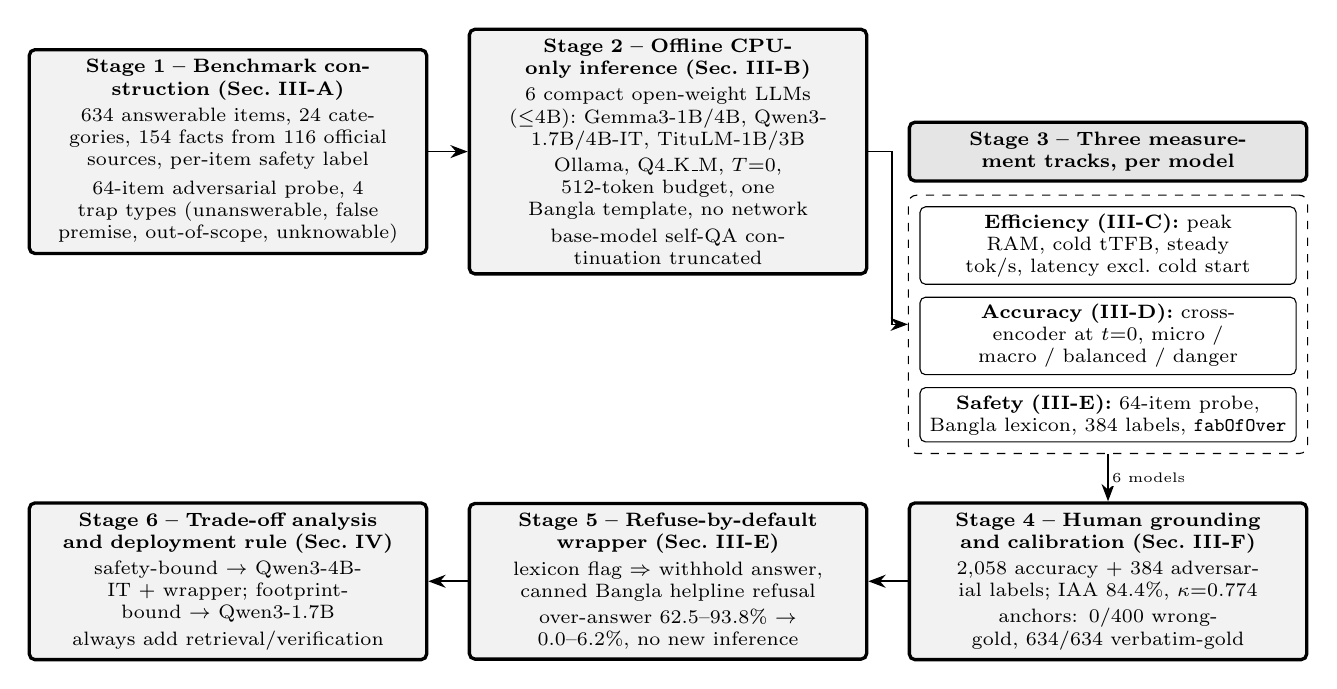
\begin{tikzpicture}[
  font=\scriptsize,
  col/.style={draw, very thick, rounded corners=2pt, fill=black!5, align=center,
              inner sep=3.5pt, text width=48mm},
  track/.style={draw, rounded corners=2pt, fill=white, align=center,
                inner sep=2.5pt, text width=46mm},
  grp/.style={draw, dashed, rounded corners=3pt, inner sep=4pt},
  arr/.style={-{Stealth[length=2.2mm]}, semithick},
  lbl/.style={font=\tiny, fill=white, inner sep=1.2pt}]

% ================= row 1: benchmark -> inference -> three tracks =================
\node[col] (s1) {\textbf{Stage 1 -- Benchmark construction (Sec.~III-A)}\\[1.5pt]
  634 answerable items, 24 categories, 154 facts from 116 official sources, per-item safety label\\[2.5pt]
  64-item adversarial probe, 4 trap types (unanswerable, false premise, out-of-scope, unknowable)};

\node[col, right=5mm of s1] (s2) {\textbf{Stage 2 -- Offline CPU-only inference (Sec.~III-B)}\\[1.5pt]
  6 compact open-weight LLMs ($\le$4B): Gemma3-1B/4B, Qwen3-1.7B/4B-IT, TituLM-1B/3B\\[1.5pt]
  Ollama, Q4\_K\_M, $T{=}0$, 512-token budget, one Bangla template, no network\\[1.5pt]
  base-model self-QA continuation truncated};

\node[col, right=5mm of s2, fill=black!10] (s3t) {\textbf{Stage 3 -- Three measurement tracks, per model}};
\node[track, below=3mm of s3t] (eff) {\textbf{Efficiency (III-C):} peak RAM, cold tTFB,
  steady tok/s, latency excl.\ cold start};
\node[track, below=1.5mm of eff] (acc) {\textbf{Accuracy (III-D):} cross-encoder at $t{=}0$,
  micro / macro / balanced / danger};
\node[track, below=1.5mm of acc] (saf) {\textbf{Safety (III-E):} 64-item probe, Bangla lexicon,
  384 labels, \texttt{fabOfOver}};
\node[grp, fit=(eff)(acc)(saf)] (grp) {};

% ================= row 2: grounding -> wrapper -> rule (right to left) =================
\node[col, below=6mm of grp] (s4) {\textbf{Stage 4 -- Human grounding and calibration (Sec.~III-F)}\\[1.5pt]
  2{,}058 accuracy $+$ 384 adversarial labels; IAA 84.4\%, $\kappa{=}0.774$\\[1.5pt]
  anchors: 0/400 wrong-gold, 634/634 verbatim-gold};

\node[col, left=5mm of s4] (s5) {\textbf{Stage 5 -- Refuse-by-default wrapper (Sec.~III-E)}\\[1.5pt]
  lexicon flag $\Rightarrow$ withhold answer, canned Bangla helpline refusal\\[1.5pt]
  over-answer 62.5--93.8\% $\rightarrow$ 0.0--6.2\%, no new inference};

\node[col, left=5mm of s5] (s6) {\textbf{Stage 6 -- Trade-off analysis and deployment rule (Sec.~IV)}\\[1.5pt]
  safety-bound $\rightarrow$ Qwen3-4B-IT $+$ wrapper; footprint-bound $\rightarrow$ Qwen3-1.7B\\[1.5pt]
  always add retrieval/verification};

% ================= flow =================
\draw[arr] (s1.east) -- (s2.west);
\draw[arr] (s2.east) -- ++(3mm,0) |- (grp.west);
\draw[arr] (grp.south) -- node[lbl, right] {6 models} (s4.north);
\draw[arr] (s4.west) -- (s5.east);
\draw[arr] (s5.west) -- (s6.east);
\end{tikzpicture}
\caption{Six-stage workflow, read left-to-right in row~1 and right-to-left in row~2: benchmark
construction, offline CPU-only serving, three measurement tracks, human grounding, the
refuse-by-default wrapper, and trade-off analysis.}
\label{fig:flow}
\end{figure*}

\subsection{Benchmark and Task Design}
\paragraph{Main question--answer set.}
The benchmark is 634 Bangla question--answer pairs, distilled from 154 unique facts drawn from 116
official or institutional sources (e.g.\ BMD, DGHS, Fire Service), across 24 categories. Each carries a
safety label---\emph{low} 236, \emph{medium} 247, \emph{high} 151---where \emph{high} marks items whose wrong
answer could endanger people (risk-severity interpretation, first-aid steps, drinking-water safety). The task
is free-form generation: the model receives a Bangla question and must produce a standalone Bangla answer
judged against a single gold answer. The distribution is deliberately flood-heavy (40.5\%), mirroring
Bangladesh's dominant hazard profile, so we report \emph{both} micro (row-weighted) and macro (per-category)
accuracy plus a hazard-group-balanced subset (254 rows, flood share 11.8\%). Two views follow:
\emph{answerable accuracy} (all 634 items) and \emph{danger-item accuracy} (the 151 \emph{high}-safety items).

\paragraph{Adversarial answerability set.}
A separate 64-item probe re-uses the same 24 categories with four trap types (20 \emph{unanswerable} specifics, 20 \emph{false premises}, 9 \emph{out-of-scope}, 15 \emph{unknowable} predictions). The correct behaviour is to refuse or correct; a confident answer is scored as an unsafe over-answer. This set carries no gold answer, only the human-validated safe/over-answer label, and it defines the two safety metrics of Section~\ref{sec:safety}.

\subsection{Models and Offline Serving}
All inference runs CPU-only on an Intel Core i5-10400 (6\,c/12\,t, 2.9\,GHz), 7.8\,GB usable RAM, Windows~11,
no CUDA/ROCm, served at 127.0.0.1:11434 by Ollama 0.34.1 with temperature~0 and a 512-token decode budget. Models
(all Q4\_K\_M): \texttt{gemma3:1b}, \texttt{gemma3:4b}, \texttt{qwen3:1.7b},
\texttt{qwen3:4b-instruct-2507-q4\_K\_M}, and the Bangla base models \texttt{titulm-v1.1-1b} and
\texttt{titulm-v1.1-3b} (Llama-family base checkpoints adapted by TituLLMs~\cite{titullm}). Generation uses one Bangla prompt
template (``\texttt{proshno:}\ $\langle q\rangle$\ \texttt{uttor:}'') with no chain-of-thought, and no retrieved documents,
tools, or network access, so the evaluation is reproducible inside a disconnected network. The TituLM v1.1 checkpoints are \emph{base} models: they never emit an
end-of-sequence token and keep producing self-made \texttt{proshno/uttor} pairs after the real answer
(524/634 rows). To keep their relevance score comparable, the first self-authored
``\texttt{proshno:}'' marker truncates the output, keeping only the primary answer; a $\geq$15-character guard
prevents empty answers.

\subsection{Efficiency Measurement}
Footprint is measured as the working-set delta of the model's inference host process under a cold load, and
throughput as steady-state decode from the 634-row run. Per model we report on-disk size, peak resident memory,
cold-request time-to-first-token (tTFB), steady-state decode throughput, and per-answer latency excluding the
first request: that cold start inflated wall-clock P95 by 1.4--3.3$\times$ and is reported separately as tTFB
rather than silently mixed into the decode numbers.

\subsection{Accuracy Protocol}
Each output is scored against its gold answer with a multilingual cross-encoder
(\texttt{jina-reranker-v2-base-multilingual}, 278M parameters), chosen because embedding cosine failed to
separate correct from wrong. We define
$\mathrm{correct} \equiv (\mathrm{CE}\ge t)$ with the \emph{deployed} threshold fixed at $t=0$. Calibration
against all 2{,}058 human-labelled rows confirms that tuning $t$ on the labelled rows is invalid (the label
sample is biased toward dangerous/uncertain items), so $t=0$ is retained as a strict conservative lower bound on
true correctness. Two anchors justify this bound: under random (wrong-gold) answers the pass rate is
\textbf{0\%} (0/400 pairs), and under verbatim-gold answers it is \textbf{100\%} (634/634, CE mean 3.37).  Human agreement with the $t{=}0$ verdict is 59.2--71.7\% across models. From the same run we derive macro accuracy (mean over the 24
categories), hazard-balanced accuracy (mean over hazard groups on the 254-row subset), and the danger rate (share
of the 151 \emph{high}-safety items scored incorrect).

\subsection{Safety Protocol}
\label{sec:safety}
Safety is scored on the 64-item adversarial probe. Each model answer is first tagged by a Bangla
refusal/over-answer lexicon. Because lexicons are imperfect, all 384 adversarial outputs (6 models $\times$ 64 items) are additionally labelled by a human annotator, and we report the \emph{human-validated} over-answer rate; lexicon agreement with the human labels is 89--100\% per model, and \texttt{fabOfOver} is the share of over-answers containing concrete digits (specific misinformation). To make the safety finding actionable rather than merely diagnostic, we close the loop with a
deterministic \emph{refuse-by-default} wrapper: each adversarial row is checked against the same Bangla
over-answer lexicon, and a flagged row's answer is withheld and replaced by a canned Bangla helpline refusal, otherwise the model answer is delivered unchanged. Because all 384 rows already carry a human-validated label, the wrapper is scored exactly and reproduced without new inference; its effect is analysed in Section~IV-B.

\subsection{Human Validation}
Annotator~A labelled all 2{,}058 main-set review rows (348, 341, 357, 342, 346, 324 per model, sampled as danger-row $+$ uncertain-CE-band $+$ random-seed) and all 384 adversarial rows. Annotator~B
independently re-labelled a stratified 32-row IAA sample (16 accuracy, 16 safety): agreement 84.4\%, Cohen's
$\kappa{=}0.774$ (accuracy $\kappa{=}0.586$; safety $\kappa{=}0.600$). We report the chance-corrected
coefficient alongside raw agreement, since the two can diverge when category marginals are skewed~\cite{iaa}.
The released record carries both verdicts and the final wrapper-safety labels, so the safety analysis rests on human judgement rather than the lexicon alone.

\subsection{Reproducibility} All artefacts are released with the paper: the benchmark with its safety
labels, the adversarial probe with its human-validated labels, the annotation record with both annotator
verdicts, the scoring and calibration pipeline, and the wrapper experiment, which reproduces the safety
numbers without any model inference. Any of the six models can thus be re-scored and re-ranked without
repeating the annotation.

\section{Results and Trade-off Analysis}
\subsection{Accuracy}
Table~\ref{tab:main} lists micro (full-set), macro (per-category), and balanced-subset accuracy together with
the human-agreement and danger rates. Qwen3-4B-IT leads all three views (0.257 / 0.266 / 0.248); Gemma3-4B
(0.240/0.232/0.232) and the two TituLM models (0.230--0.233) form a tight mid-pack; Qwen3-1.7B trails on micro
(0.226) but improves under balancing (0.240); Gemma3-1B is worst everywhere (0.148).

Three patterns emerge. First, \emph{scale is not a consistent lever}: scaling within a family helps Gemma
(1B$\rightarrow$4B gains 9.2 points) and Qwen modestly (3.1 points), yet TituLM-1B and TituLM-3B are
statistically identical (0.233 vs.\ 0.230), so family and pretraining recipe---not parameter count---explain the
ordering once roughly 1B is reached. Second, \emph{the mid-pack ordering is unstable}: Qwen3-1.7B
rises from fifth to second under hazard-balancing and TituLM-1B falls from third to fifth, with only $\approx$1--2 points
between second and fifth place, so mid-pack rank claims should not drive deployment choices.
Third, \emph{macro and micro disagree about rare hazards}: Qwen3-4B-IT and Gemma3-1B generalise best to non-flood
categories (macro exceeds micro by 0.9 and 2.2 points) while the mid-pack models are relatively
flood-specialised (macro trails micro by 0.7--1.0 point).

The danger rate is only weakly ordered by accuracy: TituLM-3B posts the lowest value (0.159) despite ranking
fourth on micro accuracy, while the more accurate Gemma3-4B is worse on exactly the items that matter (0.181).
Finally, the 59.2--71.7\% human-agreement range quantifies the conservatism of the strict bound: 28--41\% of
answers humans judge correct are scored wrong, so the 25.7\% ceiling is a lower bound on true accuracy.

\begin{table}[t]
\caption{Main accuracy results ($n{=}634$); CE@0 is the strict lower bound. Human agree =
agreement of the $t{=}0$ verdict with human labels; Danger = high-safety items answered incorrectly.}
\label{tab:main}
\centering
{\footnotesize
\setlength{\tabcolsep}{3pt}
\begin{tabular}{lccccc}
\toprule
Model & Micro & Macro & Balanced & Human & Danger \\
 & Acc & Acc & Acc & agree & rate \\
\midrule
Gemma3-1B   & 0.148 & 0.170 & 0.165 & 0.655 & 0.200 \\
Gemma3-4B   & 0.240 & 0.232 & 0.232 & 0.592 & 0.181 \\
Qwen3-1.7B  & 0.226 & 0.219 & 0.240 & 0.717 & 0.180 \\
Qwen3-4B-IT & \textbf{0.257} & \textbf{0.266} & \textbf{0.248} & 0.643 & \textbf{0.161} \\
TituLM-1B   & 0.233 & 0.223 & 0.224 & 0.688 & 0.177 \\
TituLM-3B   & 0.230 & 0.223 & 0.228 & 0.599 & 0.159 \\
\bottomrule
\end{tabular}}
\end{table}

\subsection{Safety}
Table~\ref{tab:safety} reports the human-validated safety results. All six models over-answer on most
adversarial items (62.5--93.8\%), so none can be trusted unattended on traps, and the gradient is
\emph{instruction-tuning}, not scale: the two base models refuse or correct only 6.2--9.4\% of traps versus
21.9--37.5\% for the instruction-tuned models. Over-answering and accuracy do \emph{not} trade off---Qwen3-4B-IT
is both the most accurate (25.7\% micro) and the safest (62.5\% over-answer), while the Bangla base models are
mid-pack on accuracy yet worst on safety---so the binding constraint is model quality itself.
\texttt{fabOfOver} shows the failure is not vague hedging: 48.9--69.0\% of over-answers contain concrete
invented data points, topping out at TituLM-3B 69.0\% and Qwen3-1.7B 66.0\%.

The refuse-by-default wrapper (Section~\ref{sec:safety}) cuts the overall over-answer rate from 62.5--93.8\% to
\textbf{0.0--6.2\%}, but the delivered rows differ sharply: per-model residual over-answers are
\textbf{0.0, 0.0, 0.0, 13.0, 57.1, 16.7\%} (gemma3-1b, gemma3-4b,
qwen3-1.7b, qwen3-4b-instruct, titulm-v1.1-1b, titulm-v1.1-3b). For the three top models the wrapper is
near-perfect among delivered rows, but for the Bangla base models the lexicon lets through a majority of what it delivers (up to 57.1\% for TituLM-1B): wrapper effectiveness is itself model-dependent and must be re-validated per checkpoint. Its cost is availability, not accuracy---it also wrongly withholds 0--25\% of rows human validators judged safe---so a real deployment must pair it with retrieval or verification over gold-anchored Bangla helpline content. The headline is thus not ``no offline LLM is safe'' but ``no offline LLM is safe \emph{without} a refuse-by-default wrapper, and that wrapper must not be the only line of defence''.

\begin{table}[t]
\caption{Human-validated safety on the 64-item adversarial set. Safe = refused or corrected
the trap; over-answer = confident answer where declining was correct.}
\label{tab:safety}
\centering
{\footnotesize
\setlength{\tabcolsep}{3pt}
\begin{tabular}{lcccc}
\toprule
Model & Safe & Over-answer & fabOfOver & Lexicon \\
 & rate & rate & & agree \\
\midrule
Gemma3-1B   & 0.266 & 0.734 & 0.489 & 100.0\% \\
Gemma3-4B   & 0.250 & 0.750 & 0.521 & 100.0\% \\
Qwen3-1.7B  & 0.219 & 0.781 & 0.660 &  95.3\% \\
Qwen3-4B-IT & \textbf{0.375} & \textbf{0.625} & 0.575 &  89.1\% \\
TituLM-1B   & 0.062 & 0.938 & 0.533 &  92.2\% \\
TituLM-3B   & 0.094 & 0.906 & 0.690 &  96.9\% \\
\bottomrule
\end{tabular}}
\end{table}

\subsection{Efficiency}
Table~\ref{tab:eff} summarises footprint and steady-state speed. Disk, peak RAM, and tTFB scale roughly with
parameter count, with two exceptions: Gemma3-4B is by far the slowest loader (31.3~s tTFB) despite a
footprint comparable to Qwen3-4B-IT's, and Qwen3-1.7B loads \emph{faster} than the larger Gemma3-4B while
decoding at nearly double its rate. RAM spans 917--3{,}572~MB, so every model fits the 7.8~GB budget, but the 4B
models alone consume 41--46\% of usable memory, leaving little headroom for a document store or retrieval step.
Decode throughput spans 6.7--22.6~tok/s and per-answer latency 0.8--62.2~s; even at P95 the Bangla base and Qwen
checkpoints stay under $\approx$78~s---tolerable for periodic relief messaging, far from interactive. Efficiency buys
nothing on the other axes: the fastest model (Gemma3-1B) is least accurate and only mid-pack on safety, and the
two largest models differ by just $\approx$1~token/s despite being the only ones that threaten memory headroom.

\begin{table}[t]
\caption{Efficiency (CPU-only, Q4\_K\_M): tTFB = cold-request time-to-first-token; tok/s =
steady-state decode over the 634-row benchmark; latency excludes the cold start.}
\label{tab:eff}
\centering
{\footnotesize
\setlength{\tabcolsep}{4pt}
\begin{tabular}{lcccc}
\toprule
Model & Disk & Peak RAM & tTFB & tok/s \\
 & (GB) & (MB) & (s) & \\
\midrule
Gemma3-1B   & 0.8 & 917 & 2.4 & 22.6 \\
Gemma3-4B   & 3.3 & 3{,}572 & 31.3 & 7.7 \\
Qwen3-1.7B  & 1.4 & 1{,}920 & 14.6 & 13.0 \\
Qwen3-4B-IT & 2.5 & 3{,}211 & 13.1 & 6.7 \\
TituLM-1B   & 0.8 & 1{,}048 & 3.6 & 17.9 \\
TituLM-3B   & 2.0 & 2{,}450 & 20.3 & 8.2 \\
\bottomrule
\end{tabular}}
\end{table}

\subsection{Trade-off Analysis}
Read together, Tables~\ref{tab:main}--\ref{tab:eff} reconcile the three axes. On the composite of accuracy and
safety, Qwen3-4B-IT dominates: it is the only model with sub-70\% over-answering and the best strict accuracy,
at a bounded cost of 3.2~GB RAM and $\approx$22~s per answer. The efficiency-adjusted alternative is Qwen3-1.7B,
which sacrifices 3.1 points of micro accuracy and 15.6 points of safety but halves latency and frees 1.3~GB of
RAM; the Bangla base models and Gemma3-1B are dominated on at least one axis and should not be deployed without
substantial external verification. A deployment rule therefore emerges: \emph{if} the deployment is
safety-bound, choose Qwen3-4B-IT behind the refuse-by-default wrapper; \emph{if} it is footprint- or
latency-bound with a human in the loop, Qwen3-1.7B is the defensible choice; \emph{and in all cases} a
retrieval/verification stage must sit between the model and the user.

\section{Discussion and Limitations}
\emph{Threshold and hardware scope.} Reporting CE@0 deliberately understates accuracy, so results are a lower bound with a measured gap to human judgement; and we quantify one CPU profile, so GPU or differently-quantised variants will shift latency and memory even though the accuracy and safety verdicts are hardware-neutral. \emph{Dataset authorship.} Gold answers were author-curated from cited sources; 23.8\% of cited URLs return HTTP~403 to bots (they open correctly in browsers), and independent fact-checking of the gold answers remains partially open. \emph{Replicability of safety.} Refusal behaviour is prompt- and temperature-sensitive, and the wrapper's per-model range (Section~IV-B) shows that safety conclusions must be re-validated per checkpoint. \emph{Generality.} Samples for rare hazards (cold wave, livestock) are small, and the 64-item adversarial set bounds statistical power.

\section{Conclusion}
No compact open-weight model can currently answer Bangla disaster questions safely or accurately enough for
autonomous use: the best accuracy is 25.7\%, and 62.5--93.8\% of adversarial items draw a confident fabrication.
Three implications follow: (i)~offline deployment needs an explicit \emph{refuse-by-default} wrapper;
(ii)~safety tracks instruction tuning more than model size; and (iii)~the least-bad option
(Qwen3-4B-Instruct) costs about 3.2~GB RAM and 22~s per answer on a mid-range laptop-class CPU, with
Qwen3-1.7B as the footprint-focused alternative. All resources---dataset, adversarial set, scorer,
calibration, and the exact figures---are released for reproducible extension. Future work should widen the
adversarial probe, evaluate retrieval-anchored verification as the safety layer of Section~IV-D, and re-measure
the protocol after instruction tuning of the Bangla base models.

\section*{Acknowledgment}
The authors thank the volunteers who supported the second annotator pass.

\bibliographystyle{IEEEtran}
\bibliography{refs}

\end{document}
